\section{Flanger}
\label{sec:flanger}

Flanging is an audio effect produced by mixing two identical signals together, where one signal is delayed by a small and gradually changing period.
It gets its name from the original analog method of running two tape machines slightly out of sync in respect to each other.
It is based on the principle of constructive and destructive interference of signals.

\subsection{Frequency response}\label{sec:combfilt}

A clear comprehension of the flanger, from a perceptive point of view, is highlighted by the frequency response of the comb filter.
At the heart of the algorithm, comb filter is the simplest example of a recursive delay network.
In fact, the flanger is a recursive comb filter with an interpolating and time-varying delay line.
Changes in delay time correspond to the characteristic way peaks in the frequency response move up and down in frequency~\cite{puckette2006theory}.

The comb filter is obtained by feeding a $g_{FB}$ fraction of the output back to the input. Its typical difference equation is:
\[
y[n] = g_{FB} \, y[n - M[n]] + x[n] + (g_{FF} - g_{FB}) \, x[n - M[n]],
\]
where $g_{FF}$ is the \emph{depth} of the flanger, and $M[n]$ is a function describing variable delay times.

In the flanger case, it is represented by a Low Frequency Oscillator, for each channel, of different and selectable waveforms. Thus, the frequency response of the flanger is equal to:
\[
	H[z] = \frac{1 + z^{
			-M[n]} \, \left( g_{FF} - g_{FB} \right)
	}{
		1 - z^{-M[n]} \, g_{FB}
	}
\]

By looking at the absolute value of the frequency response of the non-recirculating comb filter with $g_{FB} = 0$
\[
|H(z)| = \sqrt{ 1 + 2g_{FF} cos(\omega M[n]) + g_{FF}^2}
\]
we can appreciate the classical spectrum with peaks and notches lying respectively in 
\[
\omega_p = \frac{2 \pi p}{M} \qquad  p = 0, 1, 2, \dots, M-1
\]
and 
\[
\omega_n = \frac{(2n+1) \pi}{M} \qquad n = 0, 1, 2, \dots, M-1
\]

It is easy to see the dependence between enhanced frequencies and delay times of the flanger. The flanger is stable while $g_{FB} < 1$.

\begin{figure}
	\centering
	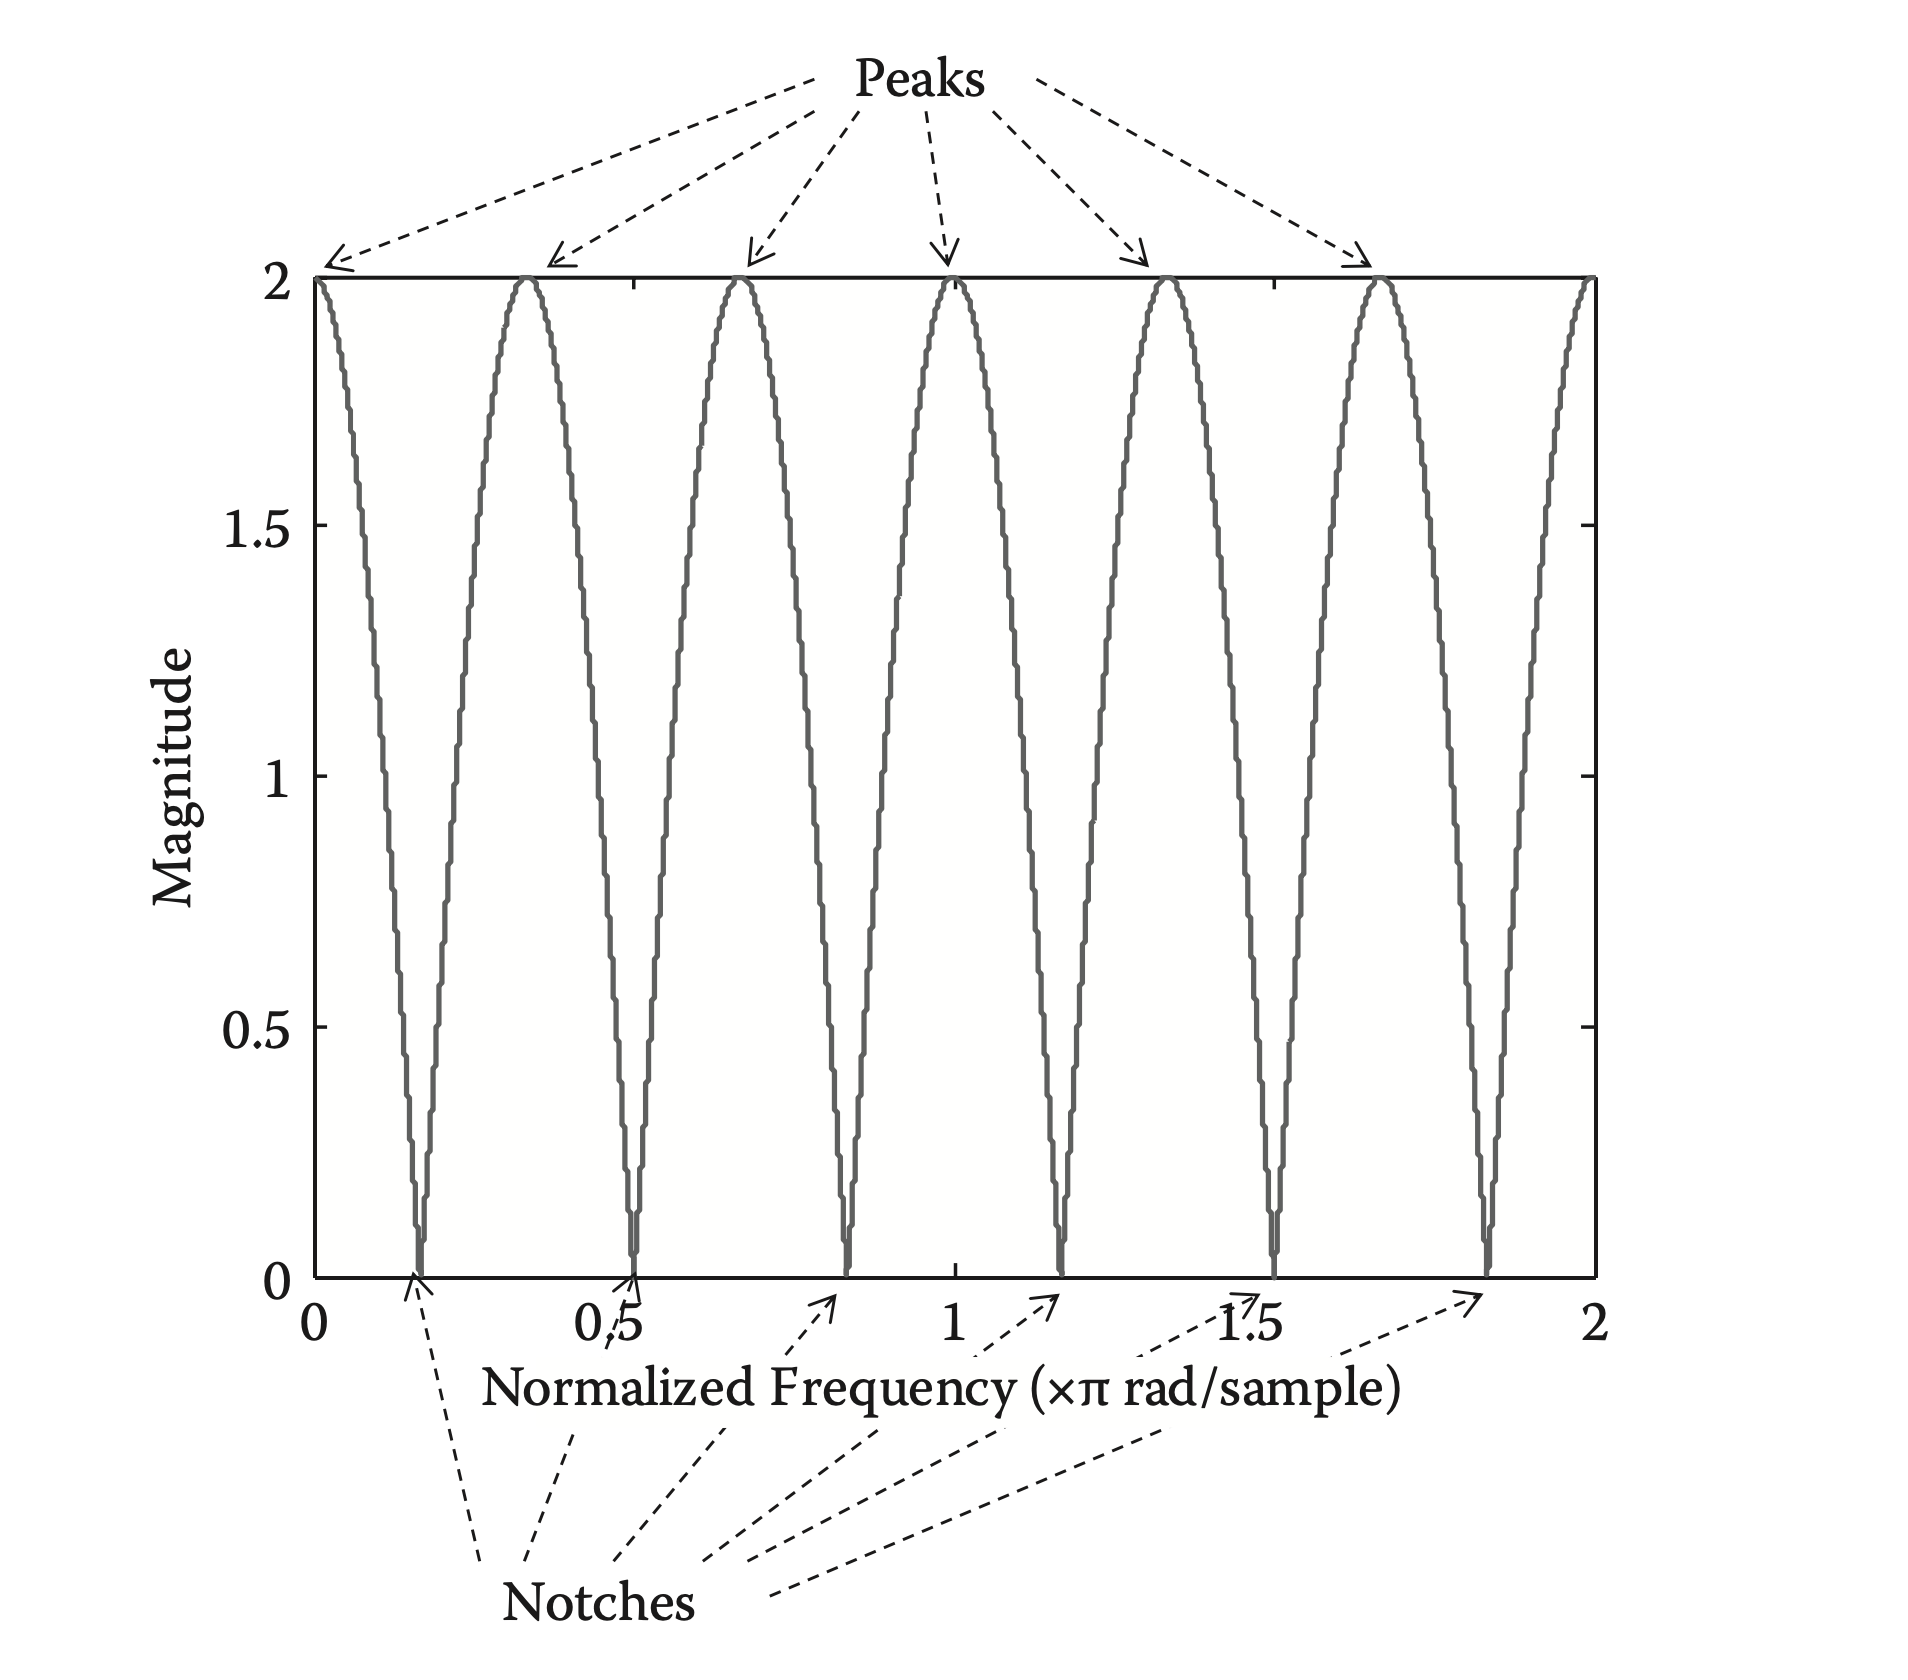
\includegraphics[width=0.5\linewidth]{assets/comb.png}
	\caption{Frequency response of a flanger}
	\label{fig:comb}
\end{figure}

Our plug-in provides the feature to invert the polarity of the $g_{FF}$ parameter. In this case, peaks and notches in the frequency response will trade places, with the first notch lying at $DC$ frequency. Because of it, when switching to the negative polarity you can hear a thinner sound unless $M$ is large.

\subsection{Implementation}\label{sec:implementation}

In order to reproduce the analog effect of the flanger given by the heads of the tape machine, a delay line with a read and a write pointer must be implemented. In the code we defined them as two variables $dr$ and $dw$. The read index moves away from, then back to, the top or starting point of the delay. When the read pointer and the write one are superimposed there is no delay, while when they are moving in respect to each other there is a change of pitch. Looking at the algorithm, a loop over all samples is implemented to calculate, for each iteration, the distance between the two pointers and store the delay length into a buffer. More details can be seen in the comments of the code.

As can be seen from the block diagram in figure~\ref{fig:diag}, our plug-in has a mono input that is duplicated and in a stereo output.
The wet lines are previously filtered by a high-pass filter (described in section~\ref{sec:hpf}) and then sent to the delay blocks. They are controlled by two distinct LFOs for each channel, with an adjustable relative phase to spread the stereo image. At the end, the wet and the dry lines are summed up to provide the two outputs $y_L[n]$ and $y_R[n]$. 

\begin{figure}
	\centering
	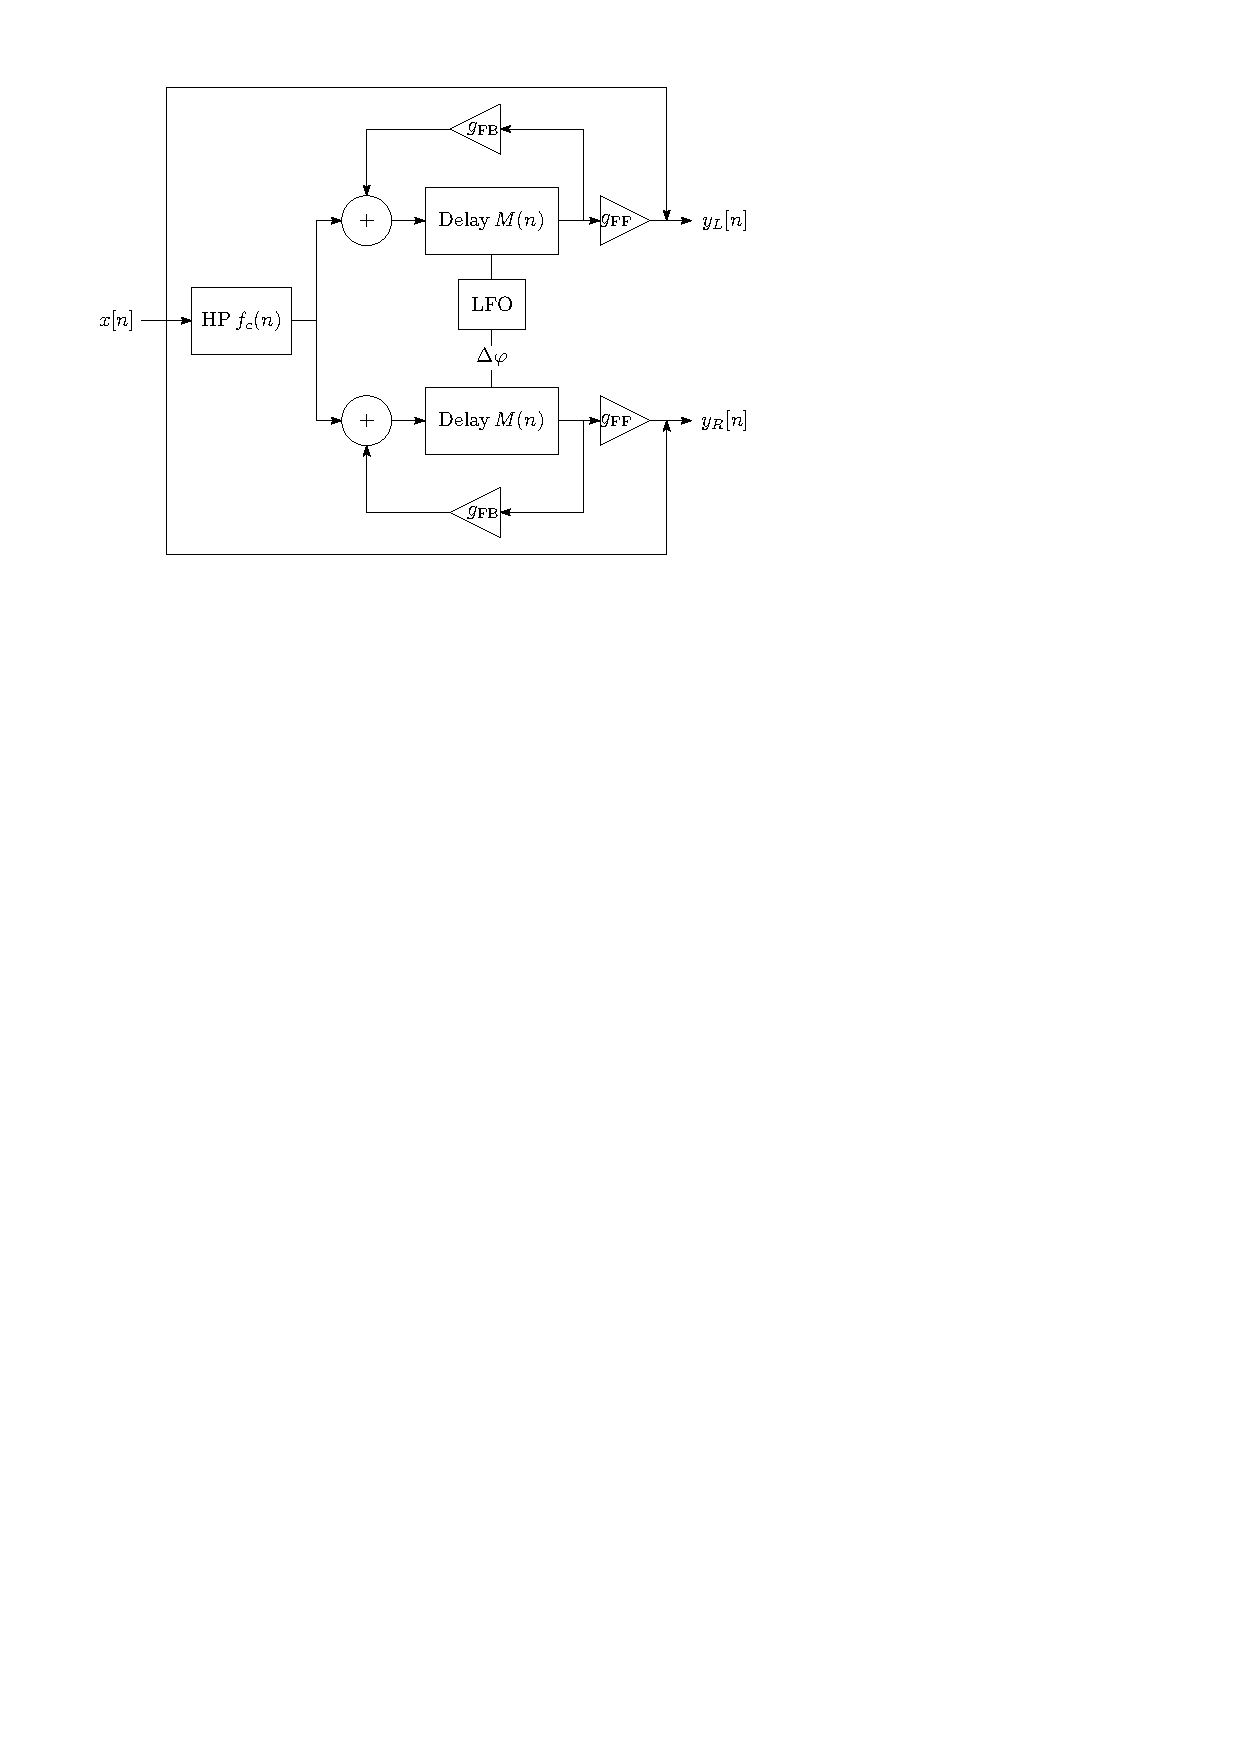
\includegraphics[width=0.7\linewidth]{assets/diagram-full.pdf}
	\caption{Complete flanger block diagram}
	\label{fig:diag}
\end{figure}

\subsection{Parameters}\label{sec:parameters}

The flanger effect is given precisely by the mix of the dry signal and the wet one (in fact if only the signal with modulated delay were sent out, we would have a sort of simple frequency modulation that would lead to a vibrato effect). In short, mixing an audio signal with a slightly delayed copy of itself results in a different frequency spectrum due to the suppression of some wave components and the enhancement of others.

\paragraph{Depth}
The mixing ratio between the two signals is a fundamental aspect of this type of effect. The control of the \emph{depth} value, expressed in percentage, is used to decide the amount of wet signal to mix to the dry one. In particular 0\% corresponds to $g_{FF} = 0$ and produces no effects, while 100\% guarantees the maximum effect.

\paragraph{Feedback}
Another user adjustable parameter is the value of the \emph{feedback gain}. It is expressed in percentage as well.
%In particular, setting this value to 0\% creates a flanger without feedback.
We decided to set the range of this parameter from 0 to 99\% to remain in a stable condition and prevent the risk of distortion of the sound.

\paragraph{Low Frequency Oscillators}
As said before, each delay line is controlled by an LFO.
We decided to set another degree of freedom for the user and we introduced some other user-adjustable parameters related to it.
In particular \emph{sweep width} is the value of the amplitude of the LFO expressed in milliseconds, in a range from 0 to 25\,ms.
It is also possible to modify the \emph{LFO frequency}, from 0 to 10\,Hz.
This parameter is useful to act on the speed of the read pointer.

The plug-in also provides the possibility to choose the type of wave.
Besides the default ``sinusoidal'' wave, it is possible to set a ``square'', ``sawtooth'', ``inverse sawtooth'', ``triangular'' or a ``random'' wave.
This part, is implemented with a simple \texttt{switch} over a \texttt{OscFunction} enum in the member function \texttt{FlangerProcessor::waveForm()} in the \texttt{PluginProcessor.cpp} file.

A final parameter is the \emph{LFO phase R/L}, ranging from 0 to 360°, which allows the user to modify phase displacement in case the wave function is not random. In the latter case, this parameter is replaced by \emph{LFO width}, which is a percentage representing how much the right channel should differ from the right one, by making a linear combination between the left-channel random value and another right-channel random value.
